%%
% Report of my internship.
% It has to give an introduction to the context and explain my work.
%%
\documentclass[12px]{article}

\usepackage[noend]{algpseudocode}
\usepackage[english]{babel}
\usepackage[a4paper]{geometry}
\usepackage[hidelinks]{hyperref}

\usepackage{algorithm}
\usepackage{apacite}
\usepackage{stmaryrd}
\usepackage{tikz}
\usepackage{todonotes}
\usepackage{wrapfig}


\begin{document}
  \section{Introduction }
    % Some bullshit is expected here I guess ?
    % Goal of the internship (maybe quickly as not everything is supposed to be introduced)
    % Technical informations about the internship, team, ...

  \section{Context and state of the art}
    % Give any information about what isn't my work
    \subsection{Union-Find algorithms}
      \subsubsection{Disjoint set structure}
        % Definition of a disjoint set structure
        The disjoint set structure is a very classical structure that represents a partition of a finite set $X = \biguplus\limits_{i \in I} S_i$. It is meant to allow three fast queries:
        \begin{itemize}
          \item $\Call{makeset}{x}$: add the element $x$ to the structure, initially in a singleton.
          \item $\Call{Union}{x, y}$: alter the structure to merge the set $x$ belongs to and the set $y$ belongs to. After such an operation, $\exists! i \in I~/~x \in S_i \land y \in S_i$.
          \item $\Call{find}{x}$: give a unique representative of the set $x$ belongs to. It means that $\forall x, y \in X,~\Call{find}{x} = \Call{find}{y} \Leftrightarrow \exists! i \in I~/~x \in S_i \land y \in S_i$.
        \end{itemize}

        In practice, it is usually represented by a forest of the elements of $X$, $\textsc{makeset}$ builds a tree containing only its root, $\textsc{union}$ merges two trees and $\textsc{find}$ returns the root of a tree given one of its nodes.
        In a program, such a forest is represented by an array of size $|X|$, assuming that $X = \llbracket 0, |X|-1 \rrbracket$, the element of index $x$ will be $y$ if $y$ is the parent of $x$ in a tree, or $x$ if $x$ is a root.

        In order to lighten notations, whenever such a structure is used, we note the parent of any node $x$ as $p(x)$.

        \begin{figure}[h]
          \caption{A disjoint set structure representing $\{\{0, 1, 2\}, \{3\}, \{4, 5\}\}$}
          \centering
          \vspace{0.2cm}
          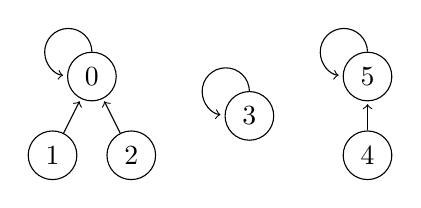
\begin{tikzpicture}[shorten >=1pt]
            \tikzstyle{vertex} = [circle, draw=black]
            \tikzstyle{legend} = [color=gray, font=\tiny]

            \node[vertex] (0) at (1, 1) {$0$};
            \node[vertex] (1) at (0.5, 0) {$1$};
            \node[vertex] (2) at (1.5, 0) {$2$};
            \node[vertex] (3) at (3, 0.5) {$3$};
            \node[vertex] (4) at (4.5, 0) {$4$};
            \node[vertex] (5) at (4.5, 1) {$5$};

            \draw [->] (0.90) arc (1:264:3mm) {};
            \draw [->] (3.90) arc (1:264:3mm) {};
            \draw [->] (5.90) arc (1:264:3mm) {};

            \draw [->] (1) -- (0);
            \draw [->] (2) -- (0);
            \draw [->] (4) -- (5);
          \end{tikzpicture}
          \hspace{1cm}
          \raisebox{0.5cm}{%
            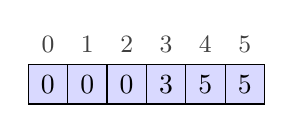
\begin{tikzpicture}[shorten >=1pt]
              \tikzstyle{value} = [draw=black, fill=blue!15, minimum width=0.5cm, minimum height=0.5cm]
              \tikzstyle{index} = [color=darkgray, font=\small]

              \foreach \i / \x in {0/0, 1/0, 2/0, 3/3, 4/5, 5/5} {%
                \node[index] at (\i / 2, 0.5) {\i};
                \node[value] at (\i / 2, 0) {\x};
              }

            \end{tikzpicture}
          }
        \end{figure}

      \subsubsection{Classical union-find algorithm}
        % Classical th. implementation of union-find, explaination why (th. complexity), applications ?
        \setlength\intextsep{0pt}
        \begin{wrapfigure}{r}{5.6cm}
          \centering
          \begin{minipage}{\linewidth}
            \begin{algorithm}[H]
              \caption{General structure of Union-Find}%
              \label{alg:union-find}
              \begin{algorithmic}[1]
                \State $F \gets \emptyset$
                \ForAll {$x \in V$}
                  \State \Call{makeset}{x}
                \EndFor
                \ForAll {$(x, y) \in E$}
                  \If {$\Call{find}{x} \neq \Call{find}{y}$}
                    \State $\Call{union}{x, y}$
                    \State $F \gets F \cup \{x, y\}$
                  \EndIf
                \EndFor
              \end{algorithmic}
            \end{algorithm}
          \end{minipage}
        \end{wrapfigure}

        A very typical application of this structure is to find a spaning forest for an undirected graph. A general algorithm used to answer this problem is called \emph{union-find} (alg.~\ref{alg:union-find}).

        Typically, \textsc{find} runs over the tree until it reaches the root, keeps track of every nodes on the path and finally set their parent to be the root. In this case \textsc{union} doesn't need to compress the trees and will just make one of the roots be parent of the other, the new root can be chosen arbitrary or given a criteria (index, rank \dots).

        This algorithm can actualy be implemented with many variations (\citeA{ufexp10}), where a typical goal is to make sure that trees never get too high, thus compressing the path leading to the root while processing \textsc{find} operation.


      \subsubsection{REM algorithm}
        % Definition and analysis of REM, explaination on why it is awesome
        \todo[noline,color=green!30,inline]{Add a reference to \emph{Dijkstra, E.W.: A Discipline of Programming}?}

        \setlength\intextsep{0pt}
        \begin{wrapfigure}[17]{r}{5cm}
          \centering
          \begin{minipage}{\linewidth}
            \begin{algorithm}[H]
              \caption{Rem's algorithm}%
              \label{alg:rem}
              \begin{algorithmic}[1]
                \State $r_x \gets x, r_y \gets y$
                \While {$p(r_x) \neq p(r_y)$}
                  \If {$p(r_x) > p(r_y)$}
                    \If {$r_x = p(r_x)$}
                      \State $p(r_x) \gets p(r_y)$
                      \State \Return false
                    \EndIf
                    \State $p_{r_x} \gets p(r_x)$
                    \State $p(r_x) \gets p(r_y)$
                    \State $r_x \gets p_{r_x}$
                  \Else
                    \If {$r_y = p(r_y)$}
                      \State $p(r_y) \gets p(r_x)$
                      \State \Return false
                    \EndIf
                    \State $p_{r_y} \gets p(r_y)$
                    \State $p(r_y) \gets p(r_x)$
                    \State $r_y \gets p_{r_y}$
                  \EndIf
                \EndWhile
                \State \Return true
              \end{algorithmic}
            \end{algorithm}
          \end{minipage}
        \end{wrapfigure}

        A familly of variation, called \emph{interleaved algorithms} in \citeA{ufexp10} replaces the two separate find operations at line 5 of Union-Find (alg.~\ref{alg:union-find}). This kind of algorithm will instead operate by running over the forest simultaneously from the two starting nodes. The first advantage of this kind of algorithm is that it won't need to reach both roots on every case.

      In Rem's algorithm, line 5 and 6 of algorithm~\ref{alg:union-find} are replaced by algorithm~\ref{alg:rem} which handles find operations, merging components if they are disconnected and compression in one loop.

      A union-find algorithm can typically be implemented to fit a worst case complexity of $O(n + m \cdot \alpha(m, n))$ where $\alpha$ is the inverse of Ackermann's function, $n = |V|$ and $m = |E|$. Rem's algorithm however, has a worst case complexity in $O(n + m^2)$.
      \todo[color=blue!30,fancyline]{Reference or proof}

    \subsection{Distributed algorithms}
      % Introduction to distributed algorithmic, existing implementation
      Almost no work seems to previously focus on the issue of distributing the union-find algorithm.
      This may be due to the fact that this algorithm is close to optimal, as much for its speed as for its memory complexity.
      It is possible however that because of the size of the input graph, the nodes don't fit in memory, \citeA{ufdist09} mentioned that an application to Hessian matrices can reach this limit.

      \subsubsection{Idea}
        \citeA{ufdist09} introduced an parallization of the algorithm, based on an approach close to REM\@.
        The same kind of zigzag merge operation is done by comparing the rank of $r_x$ and $r_y$, where the rank is the depth of a node in its component's tree.
        This process is extended to a distributed implementation by attributing for each vertex an unique process. Then, a disjoint-set structure will be stored among processes, for any node $x$, only the owner of $x$ knows the value of $p(x)$.
        Something close to the sequential algorithm can then be executed by sending messages between processes whenever the current process can't run anymore the algorithm because it doesn't own $r_x$ or $r_y$ depending on their ranks.
      This algorithm had an issue of clarity as several specific cases had to be handled with a patch. However results showed that it was nicely scalable and where encouraging some refinement.

      \subsubsection{Repartition}
        As the operations likely to be the most time-expensive, the main goal is to reduce communication charge.
        Thus, the actual first step of a distributed union-find algorithm would be to eliminate for each processing node as much edges as possible before making any communication.

    \subsection{Shared algorithms}
      % Introduction to shared algorithmic, existing implementation
      \citeA{ufshar12} showed that REM was a very convenient algorithm to adapted for parallelized computing. As it only modifies one side of the edge during each step of the merge operation, it can very easily be implemented for several cores using locks.
      \todo[color=green!30,fancyline]{Add this algorithm somewhere}
      But as locks are slow, the paper also introduce a lock-free approach that is much quicker. This approch processes by inserting edge in the structure in a first step that doesn't try to fix concurency issues. Then, the algorithm checks that each edge that added informations to the structure is still inside a component of the structure, the algorithm restarts with the set of theses node that were not connected as input and halts when this set is empty.


  \section{Writing REM as a distributed memory algorithm}
    % Description of the algorithm, experimental results
    \setlength\intextsep{0pt}
    \begin{wrapfigure}{r}{6.5cm}
      \centering
      \begin{minipage}{\linewidth}
        \begin{algorithm}[H]
          \caption{Distributed REM algorithm}%
          \label{alg:rem_distributed}
          \begin{algorithmic}[1]
            \Function{handle}{$r_x$, $r_y$, $p$}
              \State $r_x \gets$ \Call{local-root}{$r_x$, $p$}
              \State
              \If {$p(r_x) < r_y$}
                \State send $(r_y, p(r_x))$ to $owner(r_y)$
              \ElsIf {$p(r_x) > r_y$}
                \If {$p(r_x) = r_x$}
                  \State $p(r_x) \gets r_y$
                \Else
                  \State $p_{r_x} \gets p(r_x)$
                  \State $p(r_x) \gets r_y$
                  \State send $(p_{r_x}, r_y)$ to $owner(z)$
                \EndIf
              \EndIf
            \EndFunction
         \end{algorithmic}
        \end{algorithm}
      \end{minipage}
    \end{wrapfigure}

    I started my internship by writing a distributed algorithm based on the REM algorithm. After only a few versions, it appeared that it was possible to write an algorithm very close to the sequential one: executing the same conditions, where half of the decisions are to request another process.

    Each node keeps a set of pairs $(r_x, r_y)$, as in the sequential algorithm, this means that $r_x$ and $r_y$ have to be in the same component of resulting tree.
    This algorithm operate using a supersteps scheme: it will sequentially handle a chunk of edges on each processing node, then will synchronise every node and exchange datas between them and start again.

    Algorithm~\ref{alg:rem_distributed} describes how a node can handle a pair $(r_x, r_y)$.
    It runs on a node that received $(r_x, r_y)$ and expects that the sender made sure that the current node owns $r_x$. Then the algorithm runs on its knowledge of the tree by processing the ``local root'' of $r_x$ (ie.\ the highest parent of $r_x$ in the disjoint set structure maintained by this process).
    From there, the algorithm can either conclude that this edge is already inside a component of the disjoint-set structure or send a new edge to process to another node.


  \section{Mixing up distributed and shared algorithms}
    % Description of parallelized parts, experimental results


  \section{Conclusion}


  \section{Appendices}
    % Proofs, maybe extra datas
    \citeA{ufdist09}
    \citeA{ufexp10}


  \bibliographystyle{apacite}
  \bibliography{references}
\end{document}

